%%%%%%%%%%%%%%%%%%%%%%%%%%%%%%%%%%%%%%%%%%%%%%%%%%%%%%%%%%%%
%%  This Beamer template was created by Cameron Bracken.
%%  Anyone can freely use or modify it for any purpose
%%  without attribution.
%%
%%  Last Modified: January 9, 2009
%%

\documentclass[xcolor=x11names,compress]{beamer}

%% General document %%%%%%%%%%%%%%%%%%%%%%%%%%%%%%%%%%
\usepackage{booktabs}
\usepackage{graphicx}
\usepackage{epstopdf}
\epstopdfsetup{outdir=./}
\usepackage[english]{babel}
\usepackage[utf8]{inputenc}
\usepackage{tikz}
\usetikzlibrary{decorations.fractals}
%%%%%%%%%%%%%%%%%%%%%%%%%%%%%%%%%%%%%%%%%%%%%%%%%%%%%%


%% Beamer Layout %%%%%%%%%%%%%%%%%%%%%%%%%%%%%%%%%%
\useoutertheme[subsection=false,shadow]{miniframes}
\useinnertheme{default}
\usefonttheme{serif}
\usepackage{palatino}

\setbeamerfont{title like}{shape=\scshape}
\setbeamerfont{frametitle}{shape=\scshape}

\setbeamercolor*{lower separation line head}{bg=DeepSkyBlue4} 
\setbeamercolor*{normal text}{fg=black,bg=white} 
\setbeamercolor*{alerted text}{fg=red} 
\setbeamercolor*{example text}{fg=blue} 
\setbeamercolor*{structure}{fg=black} 
\setbeamercolor{block body}{bg=normal text.bg!90!black}
\setbeamercolor{block title}{fg=white,bg=normal text.bg!40!black}


\setbeamercolor*{palette tertiary}{fg=black,bg=black!10} 
\setbeamercolor*{palette quaternary}{fg=black,bg=black!10} 

\renewcommand{\(}{\begin{columns}}
\renewcommand{\)}{\end{columns}}
\newcommand{\<}[1]{\begin{column}{#1}}
\renewcommand{\>}{\end{column}}
%%%%%%%%%%%%%%%%%%%%%%%%%%%%%%%%%%%%%%%%%%%%%%%%%%




\begin{document}


%%%%%%%%%%%%%%%%%%%%%%%%%%%%%%%%%%%%%%%%%%%%%%%%%%%%%%
%%%%%%%%%%%%%%%%%%%%%%%%%%%%%%%%%%%%%%%%%%%%%%%%%%%%%%
%\section{\scshape Introduction}
\begin{frame}
\title{\large{Bayesian Networks \\ Hidden Markov Models}}
\subtitle{Description and applications}
\author{
	{\scriptsize Rafael Pérez Torres\\
	Selected Topics on Pattern Recognition\\
	Profesor: Dr. Wilfrido Gómez Flores\\
	}{\it LTI Cinvestav}\\
}
\date{
	\begin{tikzpicture}[decoration=Koch curve type 2] 
		\draw[DeepSkyBlue4] decorate{ decorate{ decorate{ (0,0) -- (3,0) }}}; 
	\end{tikzpicture}  
	\\
	\vspace{0.2cm}
	Jun 19th, 2015
}
\titlepage
\end{frame}

%%%%%%%%%%%%%%%%%%%%%%%%%%%%%%%%%%%%%%%%%%%%%%%%%%%%%%
%%%%%%%%%%%%%%%%%%%%%%%%%%%%%%%%%%%%%%%%%%%%%%%%%%%%%%
\begin{frame}{Agenda}
\tableofcontents
\end{frame}

%%%%%%%%%%%%%%%%%%%%%%%%%%%%%%%%%%%%%%%%%%%%%%%%%%%%%%
%%%%%%%%%%%%%%%%%%%%%%%%%%%%%%%%%%%%%%%%%%%%%%%%%%%%%%
\section{\scshape Bayesian Networks}
\subsection{Introduction}
\begin{frame}{Introduction to Bayesian Networks (BN)}
\begin{itemize}
	\item Some classification techniques suffer the \emph{curse of dimensionality} because their focus on all dependencies between attributes.
	\item Other techniques (like Naïve Bayes) remove all dependencies making the model really simply.
	\item Sometimes an intermediante approach is best.
\end{itemize}
\end{frame}

\begin{frame}{Introduction to Bayesian Networks (BN) II}
\begin{itemize}
	\item Such approach can be obtained through the \emph{chain rule}:
	\begin{equation}
	p(x_1, x_2, \ldots, x_l) = p(xl | x_{l-1}, \ldots, x_1)\ldots p(x_2 | x_1) p(x_1)
	\label{eq:regla-cadena}
	\end{equation}
	\item This rule states that the joint PDF can be expressed in terms of a product of several conditional PDFs and a marginal one.
	\item Then it is possible to select the features that will hold a conditional dependency with an attribute $x_i$, re-written as:
	\begin{equation}
	p(\mathbf{x}) = p(x_1)\prod_{i = 2}^{l}p(x_i | A_i)
	\end{equation}
	where donde $A_i \subseteq \left \{ x_{i-1}, x_{i-2}, \ldots , x_1  \right \}$
\end{itemize}
\end{frame}

\begin{frame}{Introduction to Bayesian Networks (BN) III}
\begin{itemize}
	\item For example, let $l=6$ and
	\begin{eqnarray}
p(x_6 | x_5, \ldots , x_1)	&=& p(x_6 | x_5, x_4) 	\\
p(x_5 | x_4, \ldots, x_1) 	&=& p(x_5 | x_4)		\\
p(x_4 | x_3, x_2, x_1) 		&=& p(x_4 | x_2, x_1)	\\
p(x_3 | x_2, x_1)			&=& p(x_3 | x_2)		\\
p(x_2 | x_1)				&=& p(x_2)
\end{eqnarray}
\end{itemize}

\end{frame}

\begin{frame}{Introduction to Bayesian Networks (BN) III}
\begin{itemize}
\item The assumptions made would be $A_6 = \left \{  x_5, x_4 \right \}, A_5 = \left \{  x_4 \right \}, A_4 = \left \{  x_2, x_1 \right \}, A_3 = \left \{  x_2 \right \}, A_2 = \emptyset$.
	\item Such assumptions can be represented like on the figure.
	\item $x_i$ is conditionally independent of any combination of its \emph{non-descendents} given its parents.
	\item Then Naïve Bayes can be considered a special case where $A_i = \emptyset, i = 2, \ldots, l$
\end{itemize}

\begin{figure}[h]
	\centering
	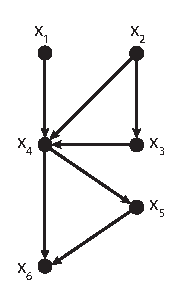
\includegraphics[scale=0.5]{../report/resources/images/dependencias-condicionales}
	\caption{Conditional dependencies}
	\label{fig:dependencias-condicionales}
\end{figure}
\end{frame}

\subsection{Definition}
\begin{frame}{BN Definition}
\begin{block}{Definition}
\begin{itemize}
	\item A BN is an directed acyclic graph (DAG) where nodes correspond to random variables (the features).
	\item Each node is associated with a set of conditional probabilities $p(x_1 | A_i)$, where $x_i$ is the variable associated with such node and $A_i$ is the set of its parents in the DAG.
	\item The full specification of a BN requires:
	\begin{enumerate}
		\item The probabilities of root nodes.
		\item The conditional probabilities  of non-root nodes.
	\end{enumerate}
	\item Joint probability is obtained multiplying such probabilities.
	\item The required work is a \emph{topological sorting} of the random variables, making that each appears before its descendents in the DAG.
\end{itemize}
\end{block}
\end{frame}

\subsection{Applications}
\begin{frame}{BN Applications}
\begin{itemize}
	\item BN have been widely employed in medical diagnosis, but is useful in any area where probability inference is needed.
\end{itemize}
\begin{figure}[h]
	\centering
	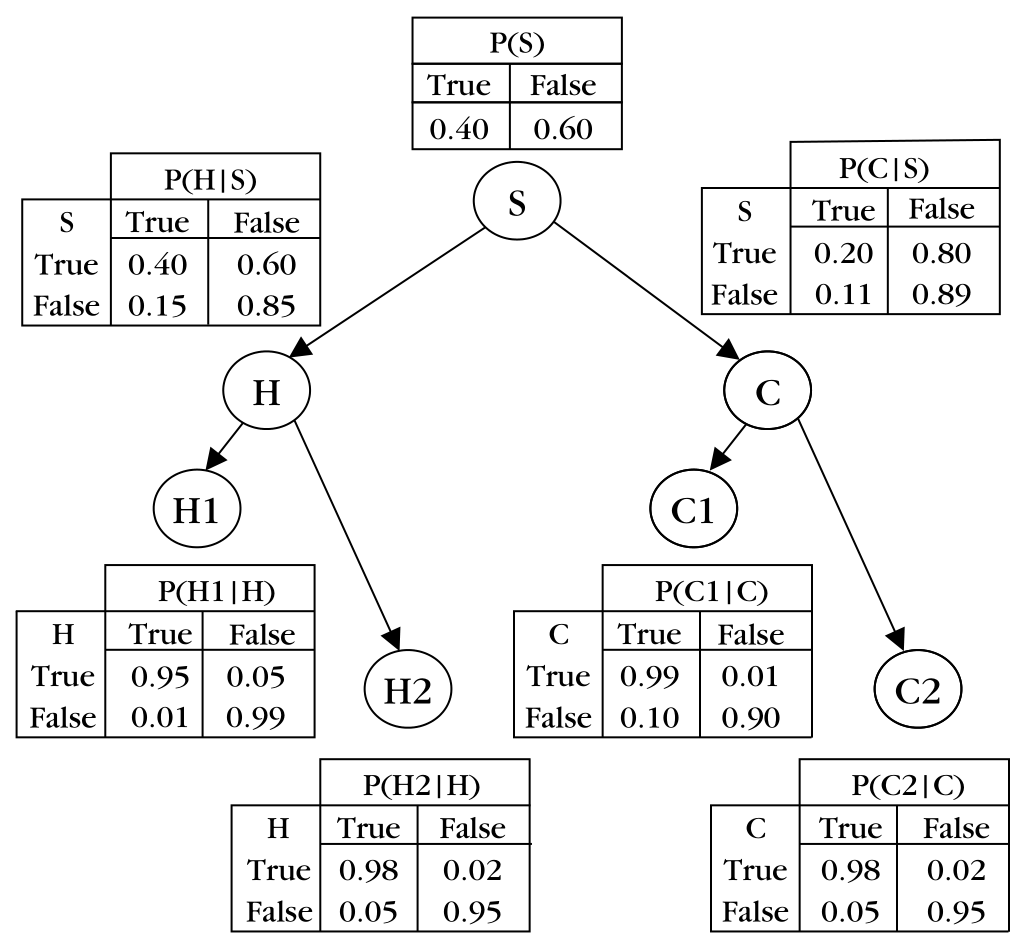
\includegraphics[scale=0.2]{../report/resources/images/ejemplo-red-bayesiana}
	\caption{BN modeling conditional dependencies for smokers (S) and their tendencies for developing cancer (C) and heart diseases (H), along associated variables for heart (H1, H2) and cancer tests (C1, C2)}
	\label{fig:ejemplo-red-bayesiana}
\end{figure}
\end{frame}

\begin{frame}{BN Training}
\begin{itemize}
	\item Structural training:
	\begin{itemize}
		\item Trees
		\item Poli-trees
		\item Multiconnected networks
	\end{itemize}
	\item Parametric training:
	\begin{itemize}
		\item Given enough data: frequency analysis.
		\item Not enough data: EM algorithm.
	\end{itemize}
\end{itemize}
\end{frame}

\section{\scshape Hidden Markov Models}
\subsection{Introduction}
\begin{frame}{Introduction to Hidden Markov Models (HMM)}
\begin{itemize}
	\item Useful when data to be analyzed come from systems where time is important.
	\item Then, the patterns are heavily linked to time.
	\item Commands given to a computer, sequence of phonems in spoken words, any event-based situation.
\end{itemize}
\end{frame}

\begin{frame}{Introduction to Hidden Markov Models (HMM) II}
Pattern types:
\begin{itemize}
	\item \textbf{Deterministic}: Generated by deterministic systems; each state depend solely on the previous state, and can be represented as a SM.
	\begin{figure}[]
	\centering
	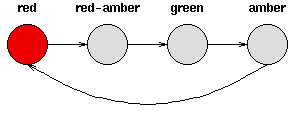
\includegraphics[scale=0.5]{../report/resources/images/traffic-lights}
	\caption{Traffic lights}
	\label{fig:semaforo}
\end{figure}
	\item \textbf{Non-deterministic}: States do not exhibit a fixed sequence. 
	However, it is still possible to make an approximation to the system.
\end{itemize}
\end{frame}


\subsection{Markov process}
\begin{frame}{Markov process}
\begin{itemize}
\item A weather model defines sunny, rainy and cloudy states.
\item We can assume that current state depends only on previous states.
\item Previous idea is the \textbf{Markov property}.
\item It is based on that \emph{Given the present, past and future are independent}.
\end{itemize}
\end{frame}

\begin{frame}{Markov process II}
\begin{itemize}
\item A Markov process moves from one state to another depending on $n$ previous states along \emph{\textbf{discrete}} time.
\item $n$ states affecting choice? \emph{$n$-order} Markov process.
\begin{figure}[h]
	\centering
	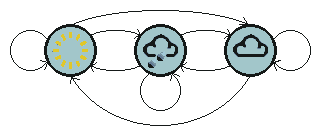
\includegraphics[scale=0.5]{../report/resources/images/weather-example}
	\caption{First order transitions on weather}
	\label{fig:transiciones-clima}
\end{figure}
\end{itemize}
\end{frame}

\begin{frame}{Markov process III}
\begin{itemize}
\item Each transition is dictated by a probability.
\item All $M^2$ probabilities build the state transition matrix .
\begin{figure}[h]
	\centering
	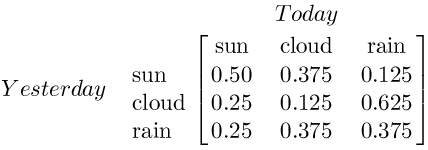
\includegraphics[scale=0.5]{../report/resources/images/weather-matrix}
	\label{fig:matriz-transicion-clima}
\end{figure}
\item Sum of each row equals 1.
\item Probabilities in initial state are given by the $\pi$ vector
\begin{figure}[tb]
	\centering
	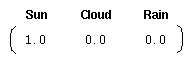
\includegraphics[scale=0.5]{../report/resources/images/pi-vector}
	\label{fig:vector-pi}
\end{figure}
\end{itemize}
\end{frame}

\begin{frame}{Markov process definition}
\begin{block}{Definition}
\begin{itemize}
\item A set of discrete states.
\item $\pi$ vector for states probability at $t_0$.
\item State transition matrix. Fixed along system execution.
\end{itemize}
Any process that can be described on this way qualifies as a Markov process.
\end{block}
\end{frame}

\subsection{Hidden Markov Models}
\begin{frame}{Hidden Markov Models}
\begin{itemize}
	\item A Markov process may not be enough to describe a system.
	\item Suppose you can not observe directly the system, but another set of input that is known to be related to the system states.
	\item For example, know the weather only from seaweed, identify a word by its speech.
	\item What is accessible is inside the \emph{visible states}.
	\item What is not accessible is inside the \emph{hidden states}.
	\item Usually, the hidden states hold the important information of the system.
\end{itemize}
\end{frame}

\begin{frame}{Hidden Markov Models II}
\begin{itemize}
	\item Amount of observable and hidden states does not need to be the same.
	\item A HMM models the link between the hidden and visible states through an Markov process hidden.
	\item Because of that it is also called a \emph{double embedded stocastic process}.
	\item An additional matrix (\emph{confusion matrix}) is needed to hold probabilities to reach a visible state from a given hidden state.
	\begin{figure}[tb]
	\centering
	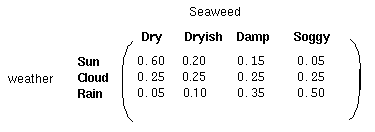
\includegraphics[scale=0.7]{../report/resources/images/weather-confusion-matrix}
	\label{fig:matriz-confusion}
\end{figure}
\end{itemize}
\end{frame}

\begin{frame}{Hidden Markov Model definition}
\begin{block}{Definition}
A HMM is a triple $(\pi,A,B)$ 
\begin{itemize}
	\item $\Pi = (\pi _i)$ vector of probabilities in initial state.
	\item $A = ( a_{ij})$ state transition matrix, holding probabilities $P(x_{i_{t}} | x_{j_{t-1}})$.
	\item $B = (b_{i_{j}})$ confusion matrix, holding probabilities $P(y_t | x_j)$
\end{itemize}
\end{block}
\end{frame}

\subsection{Applications}
\begin{frame}{Applications}
Once a system is described through an HMM, three applications can be given to it.
\begin{itemize}
	\item Evaluation
	\item Decoding
	\item Learning
\end{itemize}
\end{frame}

\begin{frame}{Evaluation}
\begin{block}{Evaluation}
Given a set of HMM (several triple $(\pi,A,B)$) describing different systems, and a sequence of observations we need to know which HMM is the most probable to have generated such sequence.
\begin{itemize}
	\item A HMM for summer, another for winter.
	\item Recognize a word from a given speech.
\end{itemize}

The forward algorithm is widely employed to solve this problem.
\end{block}
\end{frame}

\begin{frame}{Decoding}
\begin{block}{Decoding}
Finding the most probable sequence of hidden states given some observations.

The example of seaweed and weather falls in this category.

The Viterbi algorithm is employed for solving this problem.
A widely usage of Viterbi algorithm is on the NLP (Natural Language Processing) for tagging words according to its syntactic class (verb, noun, \ldots).
\end{block}
\end{frame}

\begin{frame}{Learning}
\begin{block}{Learning}
Generating a HMM from a sequence of observations.

Given  a sequence of observations (from a known set), known to represent a set of hidden states, fit the most probable HMM; that is, determine the $(\pi,A,B)$ triple that most probably describes what is seen.

The forward-backward algorithm is helpful to approximate a solution for this problem.
\end{block}
\end{frame}

\begin{frame}
\begin{block}{-}
Thank you!
\end{block}
\end{frame}

\end{document}
